\documentclass{article}
\usepackage{enumerate}
\usepackage{amsmath}
\usepackage{amssymb}
\usepackage{graphicx}
\usepackage{subfigure}
\usepackage{geometry}
\usepackage{color}
\usepackage{bm}
\usepackage{indentfirst}
\usepackage{array}

\begin{document}

\vspace*{0.25cm}

\hrulefill

\thispagestyle{empty}

\begin{center}
\begin{large}
\sc{UM--SJTU Joint Institute \vspace{0.3em} \\ Physics Laboratory \\(VE215)}
\end{large}

\hrulefill

\vspace*{5cm}
\begin{Large}
\sc{{Laboratory Report}}
\end{Large}

\vspace{2em}

\begin{large}
\sc{{Exercise 2
\vspace{0.5em}

Op Amp Lab
}}
\end{large}
\end{center}


\vfill

\begin{table}[h!]
\flushleft
\begin{tabular}{lll}
Name: Yihao Liu \hspace*{2em}&
ID: 515370910207\hspace*{2em}\\


\\

Date: 20 Oct 2016 

\end{tabular}
\end{table}

\hfill
\begin{tiny}
[rev. 1.0]
\end{tiny}
\newpage


\section{Goal}
Learn how to build and test a variety of circuits based on LM 741 Op Amp chip: non-inverting and inverting amplifiers with fixed gain.\\

Measure the gain of the amplifier and compare it with theoretical calculations.\\

Determine the saturated output voltage of the amplifier.

\section{Introduction}


\subsection{The gain of amplifier circuits}
The amplifier circuits are characterized by their gain values. The voltage gain is the ratio of output voltage to the input voltage in the circuit:
$$Voltage\ Gain=\frac{Output\ Voltage}{Input\ Voltage}$$

In the lab, you can use oscilloscope to measure the input and output peak-to-peak (ppk) amplitudes of the signals through two channels at the same time.

\subsection{Apparatus}
Apart from the DC source you are already familiar with in Lab 1, we are going to use function generator and oscilloscope this time.

\subsubsection{Function generator}

\begin{enumerate}
\item
“Parameter”: to change the amplitude, frequency of wave to generate\\
*Note: The amplitude here equals to half of the pp value. (i.e. If you set a wave whose amplitude is 100mV, the measured pp value would be 200 Vpp.) pp means peak to peak value.
\item
“1”/ “2”: to switch on the channel.
\end{enumerate}

\subsubsection{Oscilloscope}

\begin{enumerate}
\item
“Auto scale”: to automatically achieve an output on the screen with proper scale
\item
“Meas”: to turn on the measurement of the wave
\item
“1”/”2”: to show or hide the wave you detecting through channel 1 or 2
\end{enumerate}

\subsection{Procedure}

\subsubsection{Non-inverting amplifier}
You are going to build a non-inverting amplifier in this part.
\begin{enumerate}
\item
Build the circuit according to the figure below. $R_F =100\Omega$, $R_A=50\Omega$.\\
Note:
\begin{enumerate}[(a)]
\item
Use the power supply to provide $+V_{cc}$=+5V and $-V_{cc}$=-5V to the op amp.
\item
Use the COM port on the power supply as the ground in the schematic.
\end{enumerate}
\item
Use the function generator to generate a sine wave, and use it as the input voltage ($v_i$ in the figure above). Set the initial amplitude of the sine wave to 0.1$V_{pp}$. Use the oscilloscope to measure the output voltage ($v_o$ in the figure above).
\item
Increase the input voltage by 0.1$V_{pp}$ each time and record the corresponding output until the output voltage is saturate, which means the output voltage is not increasing any more as the input voltage increases.
\end{enumerate}

\subsubsection{Inverting amplifier}
You are going to build an inverting amplifier in this part.
\begin{enumerate}
\item
Build the circuit according to the figure below. $R_F =100\Omega$, $R_A=50\Omega$.\\
Note:
\begin{enumerate}[(a)]
\item
Use the power supply to provide $+V_{cc}$=+5V and $-V_{cc}$=-5V to the op amp.
\item
Use the COM port on the power supply as the ground in the schematic.
\end{enumerate}
\item
Use the function generator to generate a sine wave, and use it as the input voltage ($v_i$ in the figure above). Set the initial amplitude of the sine wave to 0.1$V_{pp}$. Use the oscilloscope to measure the output voltage ($v_o$ in the figure above).
\item
Increase the input voltage by 0.1$V_{pp}$ each time and record the corresponding output until the output voltage is saturate, which means the output voltage is not increasing any more as the input voltage increases.
\end{enumerate}

\section{Results and Discussion}

\subsection{Resistances and Voltage Supply}

\begin{table}[!h]
\begin{center}
\begin{tabular}{|c|c|}
\hline
$R_1[\Omega]$ & 99.5 \\
\hline
$R_2[\Omega]$ & 51.2 \\
\hline
\end{tabular}
\caption{The resistances of the two resistors we use to build the circuit.}
\label{tab-1}
\end{center}
\end{table}

\begin{table}[!h]
\begin{center}
\begin{tabular}{|c|c|}
\hline
$+V_{cc}[V]$ & 5.00 \\
\hline
$-V_{cc}[V]$ & -5.00 \\
\hline
\end{tabular}
\caption{The voltage supplied to the op amp.}
\label{tab-2}
\end{center}
\end{table}

\subsection{Non-inverting Amplifier}

\begin{table}[!h]
\begin{center}
\begin{tabular}{|c|c|}
\hline
$+V_{pp(in)}[V]$ & $V_{pp(out)}[V]$ \\
\hline
0.100	&	0.302\\
\hline
0.200	&	0.600\\
\hline
0.300	&	0.904\\
\hline
0.400	&	1.200\\
\hline
0.500	&	1.500\\
\hline
0.600	&	1.800\\
\hline
0.700	&	2.100\\
\hline
0.800	&	2.400\\
\hline
0.900	&	2.700\\
\hline
1.000	&	3.000\\
\hline
\end{tabular}
\caption{Non-inverting amplifier.}
\label{tab-3}
\end{center}
\end{table}

Use MATLAB to plot the figure.
\begin{figure}[h!]
    \centering
    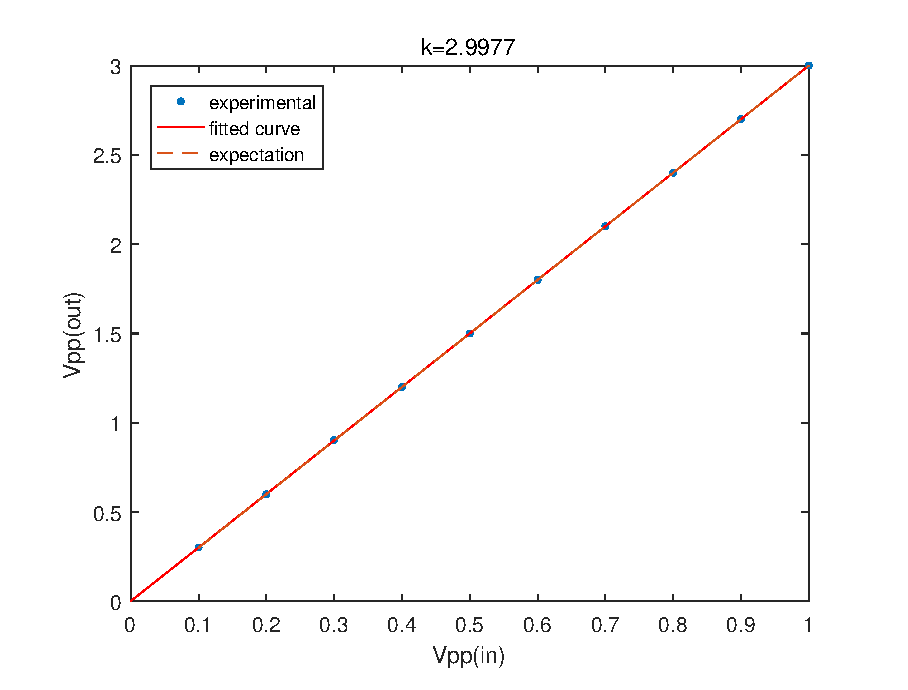
\includegraphics[width=7cm]{1.eps}
    \caption{Non-inverting amplifier.}
    \label{fig-1}
\end{figure}

We can find that 
$$\frac{V_{out}}{V_{in}}=2.9977$$

By directly calculating,
$$\frac{V_{out}}{V_{in}}=1+\frac{99.5}{51.2}=2.943$$

They are very similar.

\subsection{Inverting Amplifier}


\begin{table}[!h]
\begin{center}
\begin{tabular}{|c|c|}
\hline
$+V_{pp(in)}[V]$ & $V_{pp(out)}[V]$ \\
\hline
0.100	&	0.187\\
\hline
0.200	&	0.353\\
\hline
0.300	&	0.520\\
\hline
0.400	&	0.686\\
\hline
0.500	&	0.860\\
\hline
0.600	&	1.020\\
\hline
0.700	&	1.193\\
\hline
0.800	&	1.346\\
\hline
0.900	&	1.533\\
\hline
1.000	&	1.717\\
\hline
\end{tabular}
\caption{Inverting amplifier.}
\label{tab-3}
\end{center}
\end{table}

Use MATLAB to plot the figure.
\begin{figure}[h!]
    \centering
    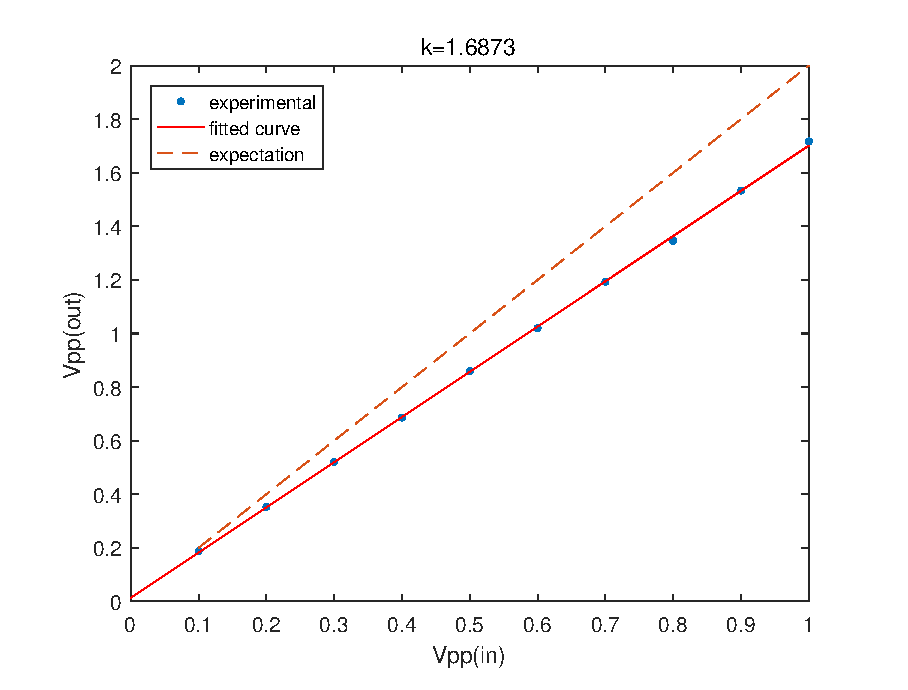
\includegraphics[width=7cm]{2.eps}
    \caption{Inverting amplifier.}
    \label{fig-1}
\end{figure}

We can find that 
$$\frac{V_{out}}{V_{in}}=1.6873$$

By directly calculating,
$$\frac{V_{out}}{V_{in}}=-\frac{99.5}{51.2}=-1.943$$

They are not similar, probably because of the resistance in the amplifier can't be neglected when it is connected as an inverting amplifier.

\section{Conclusion}
In the lab, we learned how to build and test a variety of circuits based on LM 741 Op Amp chip: non-inverting and inverting amplifiers with fixed gain.We measured the gain of the amplifier and compared it with theoretical calculations and determinef the saturated output voltage of the amplifier.

\section{Reference}
Circuits Make Sense, Alexander Ganago, Department of Electrical Engineering and Computer Science, University of Michigan, Ann Arbor.

\section{Pre-lab and Data sheet}

\end{document}